\subsection{System~1 Against LLM Judges}
\label{sec:system1}

The division gives judging to System~1.
To test it, we asked gpt-4.1-mini and DeepSeek the question \jev{} answers, with the same dialogue and records, for 599 LoCoMo and \lme{} questions (14,359 records, 1,004 of them gold evidence).
\jev{} separates gold evidence best (\cref{fig:system1}): AUC 0.942 against 0.900 for DeepSeek and 0.853 for gpt-4.1-mini, and 0.939 against 0.872 and 0.798 on \lme, whose chat-turn records rarely repeat the question's words.
A \jev{} call on 24 records takes 0.34\,s and costs \$0.00044 while answering two questions per record; DeepSeek takes 1.05\,s and \$0.00066, and gpt-4.1-mini 3.74\,s and \$0.0017, for one.
System~1 work is thus done better, and 3--11 times faster, by a System~1 model: with three to five such calls per question, several on the critical path, an LLM judge would add seconds and cost while separating evidence less well.

\begin{figure}[!htb]
\centering
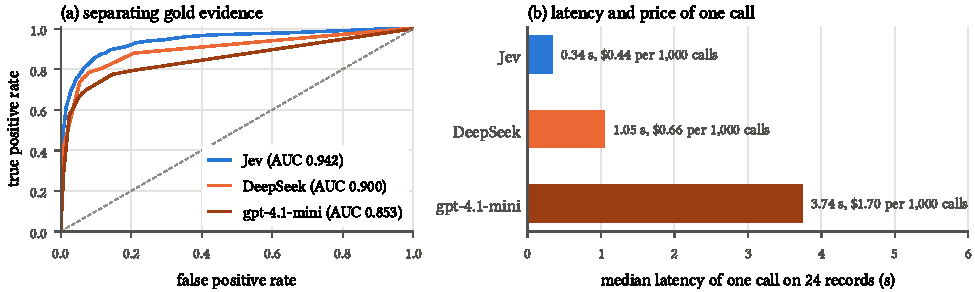
\includegraphics[width=\linewidth]{figures/system1.pdf}
\caption{\jev{} and two LLM judges on the same 14,359 records: (a) ROC curves for separating gold evidence, pooled over records; (b) median latency and list price of one call judging 24 records, in which \jev{} also answers a second question (no longer current) for every record.}
\label{fig:system1}
\end{figure}

\subsection{What Consolidation Adds}
\label{sec:consolidation}

Consolidation is the System~2 work that \sys{} moves off the path of a reply, and answering the same questions with the index removed measures what it adds.
With gpt-4.1-mini answering it adds \consLoCoMoAbs{} points on LoCoMo, \consLMEAbs{} on \lme, \consBeamAbs{} on BEAM-100K and \consBeamTenAbs{} on BEAM-10M, and \dsConsLoCoMoAbs{} on LoCoMo and \dsConsLMEAbs{} on \lme{} with the reasoning model as System~2, each with a 95\% interval above zero; on HaluMem the two judges disagree in sign.
The gains fall where a question does not point to its evidence: instruction following, knowledge updates, summarization and abstention on BEAM; knowledge updates and multi-session questions on \lme; and temporal questions, for which the timelines supply dates.
Consolidation multiplies the cost per question by \consCostRange, mostly for \jev{} to judge the index items.
